% Dieser Text ist urheberrechtlich gesch�tzt
% Er stellt einen Auszug eines von mir erstellten Referates dar
% und darf nicht gewerblich genutzt werden
% die private bzw. Studiums bezogen Nutzung ist frei
% Mai. 2007
% Autor: Sascha Frank 
% Universit�t Freiburg 
% www.informatik.uni-freiburg.de/~frank/
\documentclass{beamer}
% \documentclass[notes=only]{beamer}
\usepackage{pst-bar,pst-plot,pstricks-add}
\usepackage{graphics,graphicx}
\usepackage{pstricks,pst-node,pst-tree}
% \setbeameroption{show notes}
\setcounter{tocdepth}{1}

\setbeamertemplate{navigation symbols}{}
\beamersetuncovermixins{\opaqueness<1>{25}}{\opaqueness<2->{15}}
\usetheme{CambridgeUS}
\usecolortheme{seahorse}

\begin{document}
	\title{The max-min-hill-climbing algorithm}  
	\author[M. Bauer]{Michael Bauer}
	\institute[M.Sc. Comp. Science]{M.Sc. Comp. Science}
	\date{\today}


\begin{frame}
	\titlepage
\end{frame}
\note{
	\begin{itemize}
		\item the max-min part is a constrained-based part
		\item hill-climbing is a greedy (local) search
	\end{itemize}
}


\section{Introduction}
	\subsection{Introduction}
		\begin{frame}
			\begin{center}
				$
					\psmatrix[colsep=1.2cm,rowsep=1cm,mnode=circle]
					Difficulty&&Intelligence\\
					&Grade\\
					\endpsmatrix
				$
			\end{center}
		\end{frame}
	\note{
		\begin{itemize}
			\item What is the algorithm about?
			\item Why do we need it?
			\item Where do I start from?
			\item having a matrix (dataframe in R) with observed date which follow probabilistic distributions
			\item talk about picture
		\end{itemize}
	}

\section{Probability theory}
	\subsection{Conditional Independence}
		\begin{frame}
			\begin{block}{Definition (Conditional Independence)}
				Two variables $X$ and $Y$ are \underline{conditionally independent given \textbf{Z}} w.r.t a probability distribution P, denoted as $Ind_{p}(X;Y|\textbf{Z})$, if $\forall x,y,\textbf{z}$, where $P(\textbf{Z} = \textbf{z}) > 0$,
					\begin{equation}
						P(X,Y|\textbf{Z}) = P(X|\textbf{Z})*P(Y|\textbf{Z}),
					\end{equation}
				where $P(X,Y|\textbf{Z}) = P(X \cap Y|\textbf{Z})$. \pause \\
				It is equivalent
					\begin{equation}
						Ind(X;Y|\textbf{Z}) \Longleftrightarrow (Assoc(X;Y|\textbf{Z}) = 0),
					\end{equation}
				where $Assoc(X;Y|\textbf{Z})$ is the strength association (dependency) of $X$ and $Y$ given $\textbf{Z}$.
			\end{block}
		\end{frame}
	\note{
		\begin{itemize}
			\item \underline{Independence:} coin toss; is a useful concept but not common. Most of the time two events are independent given an additional event
			\item \underline{conditional probability:} pick a student -> intelligence -> grade
			\item \underline{conditional independence:}
			\begin{itemize}
				\item say admitted to Google, admitted to Apple
				\item in most reasonable distributions these two events are not independent
				\item assume they base their decision only on the grade
				\item we assume that (pick one) student has grade A
				\item the grade holds the relevant information
				\item Google is conditional independent of Apple given grade A
			\end{itemize}
			\item \underline{Assoc:} Do not forget about Assoc -> Min and Max
		\end{itemize}
	}

	\subsection{Graph for example}
		\begin{frame}
			\begin{center}
				$
					\psmatrix[colsep=1.2cm,rowsep=1cm,mnode=circle]
					&Grade\\
					Google&&Apple\\
					\endpsmatrix
					\ncline{->}{1,2}{2,1}
					\ncline{->}{1,2}{2,3}
				$
			\end{center}
		\end{frame}
	\note{
		\begin{itemize}
			\item DAG
			\item vertice - random variable
			\item edge - follow probability distributions
		\end{itemize}
	}

\section{Graph theory}
	\subsection{Bayesian Network}
		\begin{frame}
			\frametitle{Bayesian Networks}
				$
					\psmatrix[colsep=1.2cm,rowsep=1cm,mnode=circle]
					&parent&&parent\\
					&&child \& parent&&child\\
					&&child
					\ncline{->}{1,2}{2,3}
					\ncline{->}{1,4}{2,3}
					\ncline{->}{1,4}{2,5}
					\ncline{->}{2,3}{3,3}
					\endpsmatrix
				$
		\end{frame}

	\subsection{Blocked paths}
		\begin{frame}
			\frametitle{Blocked paths \& d-seperation}
			\begin{block}{Define three sets}
				\begin{center}
					Let $A_{1}$, $A_{2}$ and $A_{3}$ denote sets with:
					\begin{eqnarray}
						A_{1} &=& \{W\} \notag \\
						A_{2} &=& \{R, V\} \notag \\
						A_{3} &=& \{R, P\} \notag
					\end{eqnarray}
				\end{center}
			\end{block}
		\end{frame}
	\note{
		A path from X to Y is blocked by a set of nodes A if there is a node P on the path holding one of the following two conditions:
		\begin{itemize}
			\item P is not a collider and P is not in A or
			\item P is a collider and neither P or one of its descendants are in A.
		\end{itemize}
	}

		\begin{frame}
			\begin{center}
				$
					\psmatrix[colsep=1.2cm,rowsep=1cm,mnode=circle]
					X&C&Y
					\ncline{->}{1,1}{1,2}
					\ncline{->}{1,3}{1,2}
					\endpsmatrix
				$
			\end{center}
			\begin{center}
				$
					\psmatrix[colsep=1.0cm,rowsep=1cm,mnode=circle]
					X&[fillstyle=solid,fillcolor=gray]W&Y
					\ncline{->}{1,1}{1,2}
					\ncline{->}{1,3}{1,2}
					\endpsmatrix
				$
			\end{center}
			\begin{center}
				$
					\psmatrix[colsep=1.0cm,rowsep=1cm,mnode=circle]
					X&[fillstyle=solid,fillcolor=orange]R&S&T&U&[fillstyle=solid,fillcolor=orange]V&Y
					\ncline{->}{1,1}{1,2}
					\ncline{->}{1,2}{1,3}
					\ncline{->}{1,3}{1,4}
					\ncline{->}{1,7}{1,6}
					\ncline{->}{1,6}{1,5}
					\ncline{->}{1,5}{1,4}
					\endpsmatrix
				$
			\end{center}
			\begin{center}
				$
					\psmatrix[colsep=1.0cm,rowsep=1cm,mnode=circle]
					X&[fillstyle=solid,fillcolor=yellow]R&S&T&U&V&Y \\
					&W&&[fillstyle=solid,fillcolor=yellow]P&&Q
					\ncline{->}{1,1}{1,2}
					\ncline{->}{1,2}{1,3}
					\ncline{->}{1,3}{1,4}
					\ncline{->}{1,7}{1,6}
					\ncline{->}{1,6}{1,5}
					\ncline{->}{1,5}{1,4}
					\ncline{->}{1,2}{2,2}
					\ncline{->}{1,4}{2,4}
					\ncline{->}{1,6}{2,6}
					\endpsmatrix
				$
			\end{center}
		\end{frame}

\section{The algorithm}
	\subsection{How the algorithm works}
		\begin{center}
			\begin{frame}
				\begin{center}
					\begin{figure}
						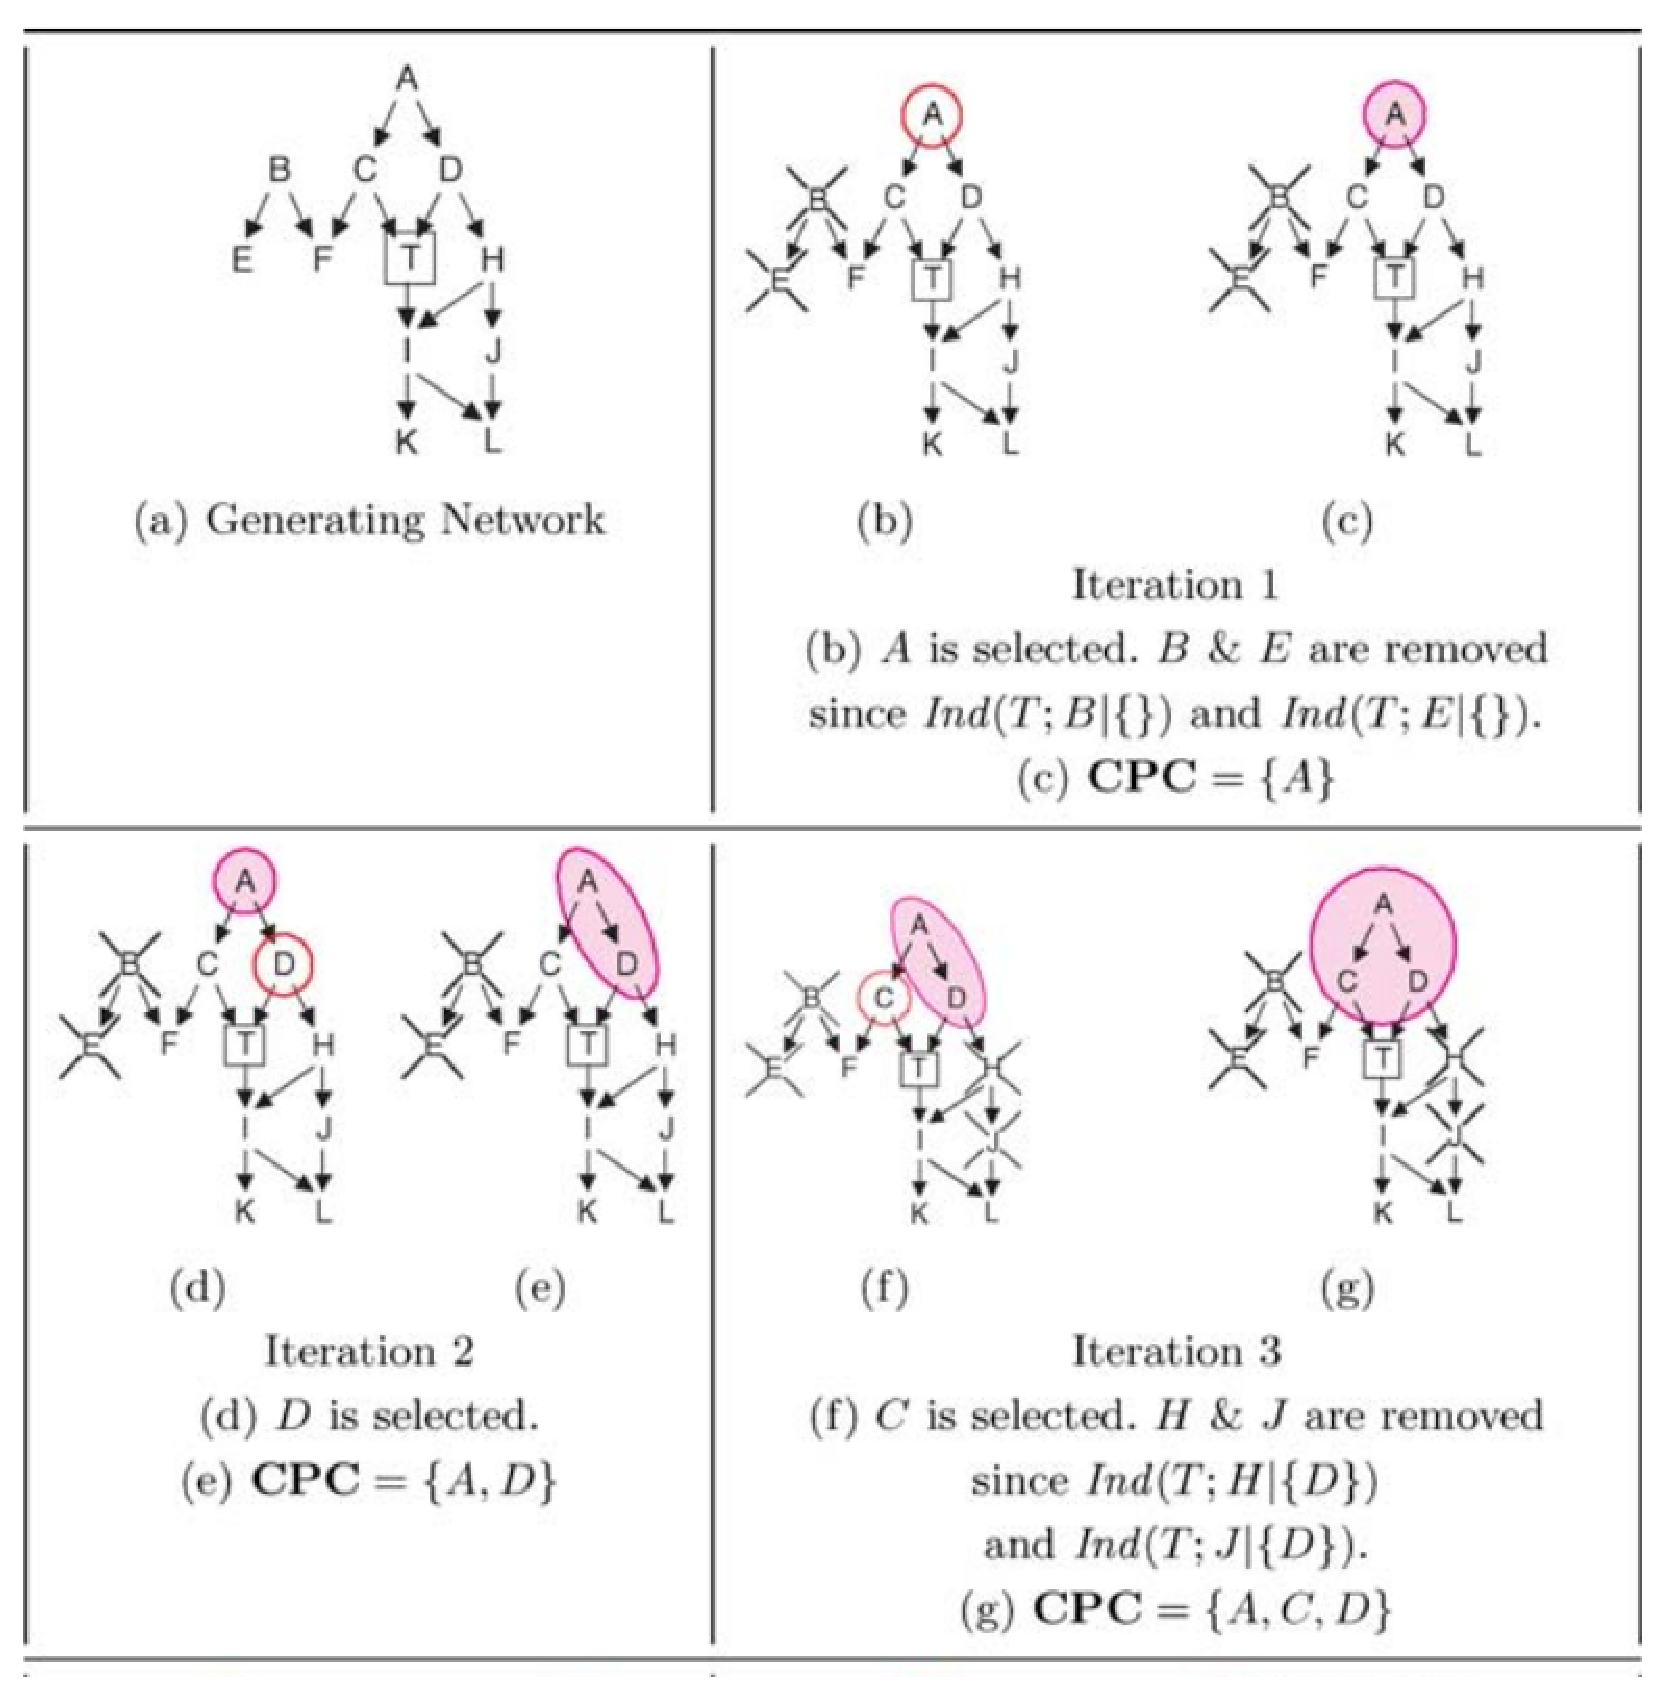
\includegraphics[scale=0.3]{img/example_part1}
					\end{figure}
				\end{center}
			\end{frame}
		\end{center}

	\subsection{How the algorithm works}
		\begin{center}
			\begin{frame}
				\begin{center}
					\begin{figure}
						\includegraphics[scale=0.4]{img/example_part2}
					\end{figure}
				\end{center}
			\end{frame}
		\end{center}

	\subsection{Thank you}
		\begin{frame}
			\begin{block}{\center{\Huge{Thanks for your attention!}}}\end{block}
		\end{frame}

\end{document}